\documentclass[pscyr,10pt]{hedlab}
\usepackage[russian]{babel}
\usepackage{graphicx}
\graphicspath{{images/}}
\usepackage[usenames,dvipsnames]{color}
\usepackage{listings}

\labnum{3}
\labname{Облако Google AppEngine}
\student{Чечеткин~И.~А.}
\date{25 ноября 2014 г.}

\lstset{
  basicstyle=\footnotesize,
  inputencoding=utf8,
  extendedchars=True,
  language=[Sharp]C,
  numbers=left,
  numberstyle=\footnotesize,
  breakatwhitespace=\false,
  breaklines=True,
  tabsize=2,
  keepspaces=true,
  escapechar=\%,
}

\definecolor{gred}{RGB}{248,203,203}
\definecolor{ggrn}{RGB}{166,243,166}

\newcommand{\hred}{\makebox[0pt][l]{\color{gred}\rule[-2pt]{\linewidth}{10pt}}}
\newcommand{\hgrn}{\makebox[0pt][l]{\color{ggrn}\rule[-2pt]{\linewidth}{10pt}}}

\begin{document}
  \makeheader
  
  \begin{center}
    \textbf{MapReduce на C\#:}
  \end{center}
  
  Исправления для работы с файлами:\\
  \begin{minipage}{.45\textwidth}
  \begin{lstlisting}
using System;
%\hred%
...
 
namespace lab4 
{
  ... 
 
  class Program 
  { 
    static void Main(string[] args) 
    {
%\hred%      var lines = new[] { 
%\hred%        "00000000000000000000", 
%\hred%        "uuuuuuuuuuuuuuuuuuuuuuuuuuuu?" 
%\hred%      };
 
      foreach (var line in lines) 
      ...
  \end{lstlisting}
  \end{minipage} \hfill
  \begin{minipage}{.45\textwidth}
  \begin{lstlisting}
using System;
%\hgrn%using System.IO;
...
 
namespace lab4 
{
  ... 
 
  class Program 
  { 
    static void Main(string[] args) 
    {
%\hgrn%      Console.WriteLine("Input path to file");
%\hgrn%      string s = Console.ReadLine();
%\hgrn%
%\hgrn%      string[] lines = File.ReadAllLines(s);
 
      foreach (var line in lines) 
      ...
  \end{lstlisting}
  \end{minipage}

  Результат работы:
  \begin{figure}[h!]
    \center
    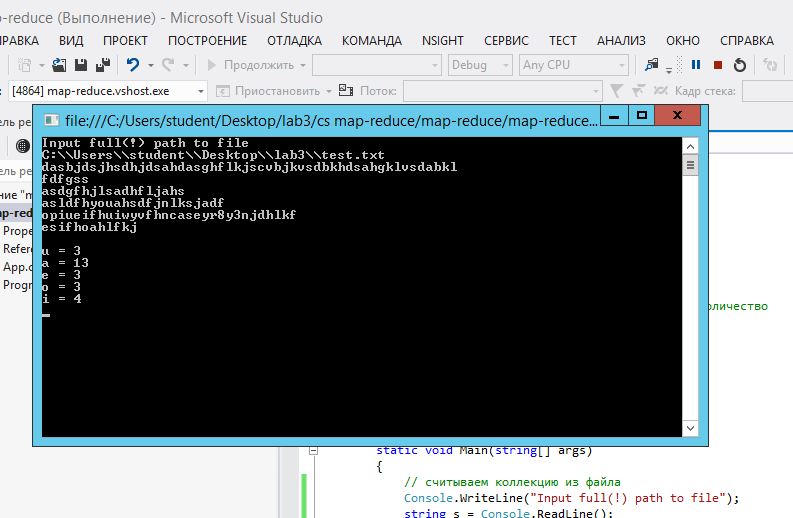
\includegraphics[width=.95\textwidth]{00}
  \end{figure}
  
  \newpage  
  \begin{center}
    \textbf{Hello world}
  \end{center}
  
  \begin{figure}[h!]
    \center
    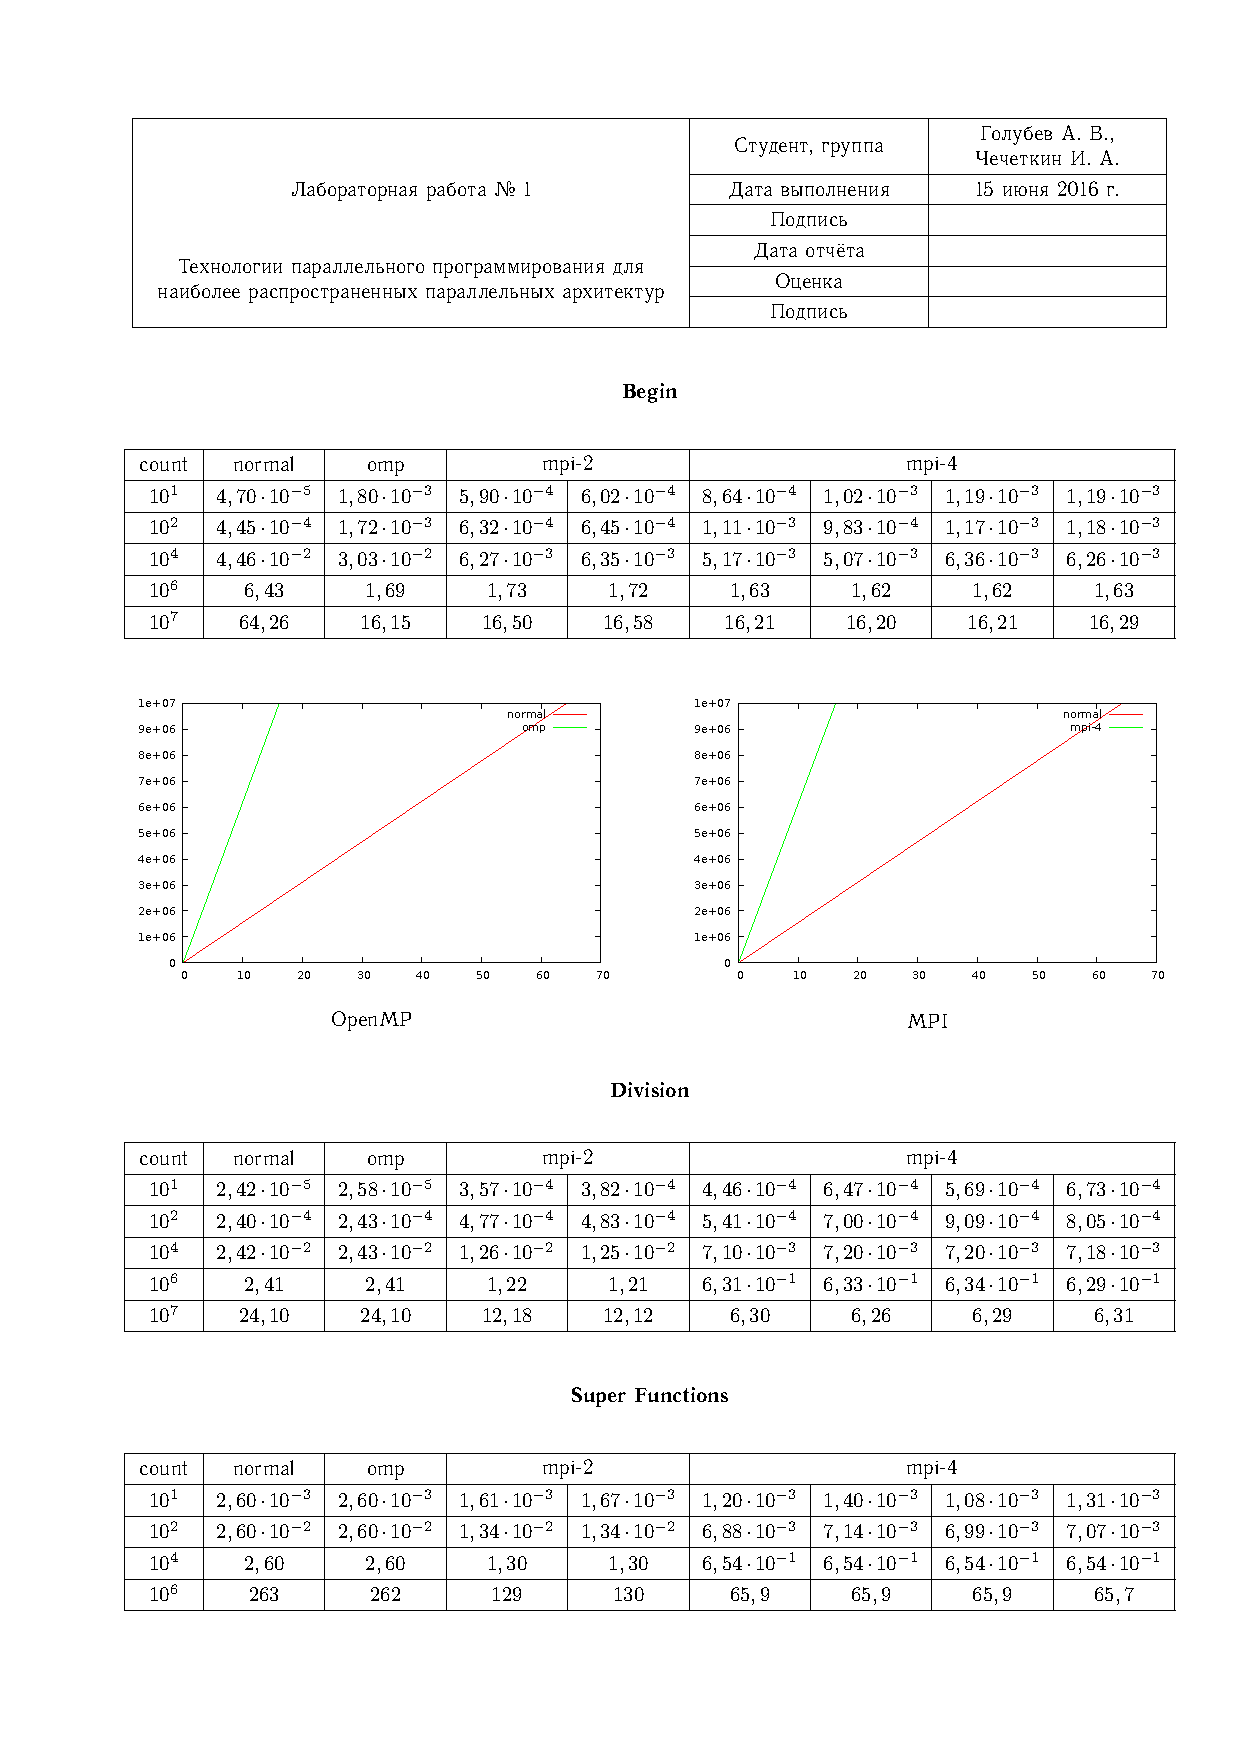
\includegraphics[width=.47\textwidth]{01} \hfill
    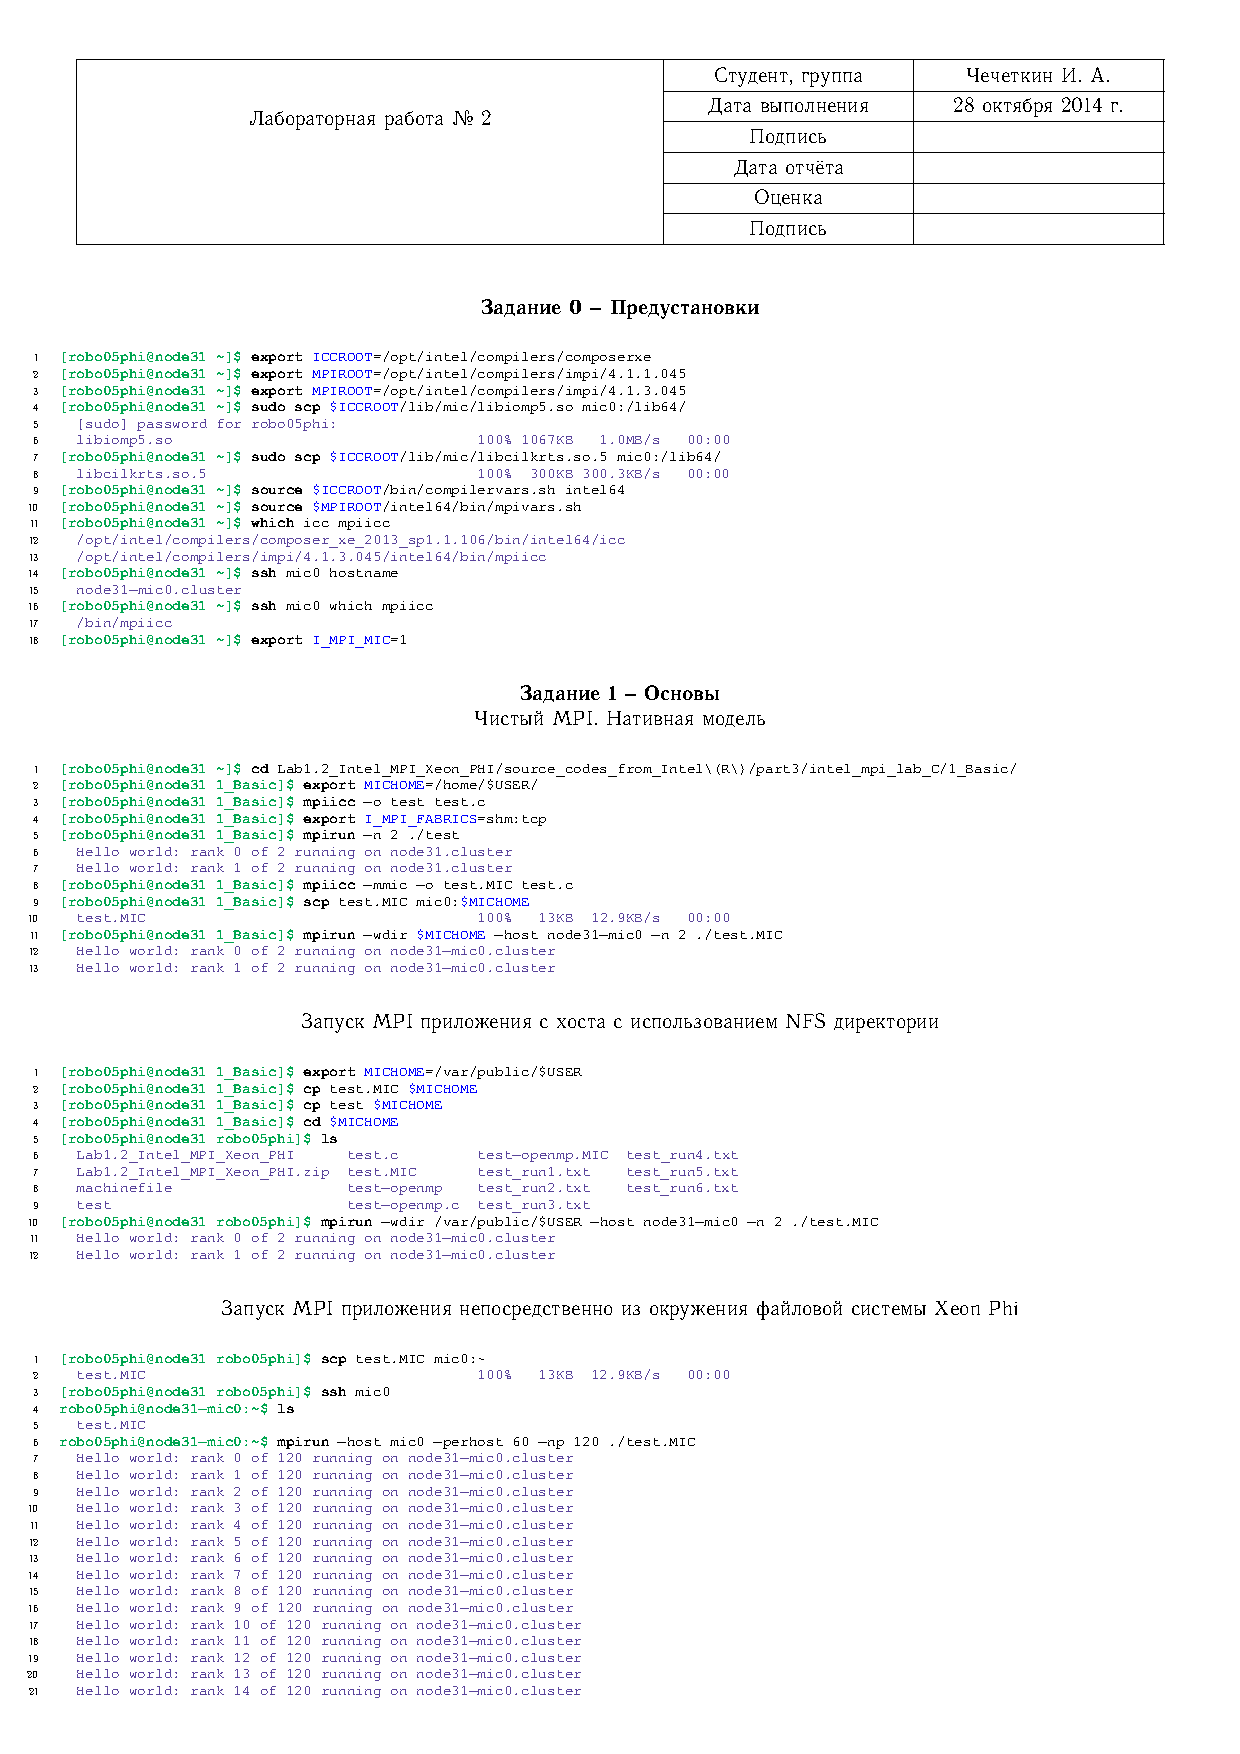
\includegraphics[width=.47\textwidth]{02}
    \parbox{.47\textwidth}{\center Окно Google App Engine Launcher} \hfill
    \parbox{.47\textwidth}{\center Hello World на localhost}
  \end{figure}
  
  \begin{figure}[h!]
    \center
    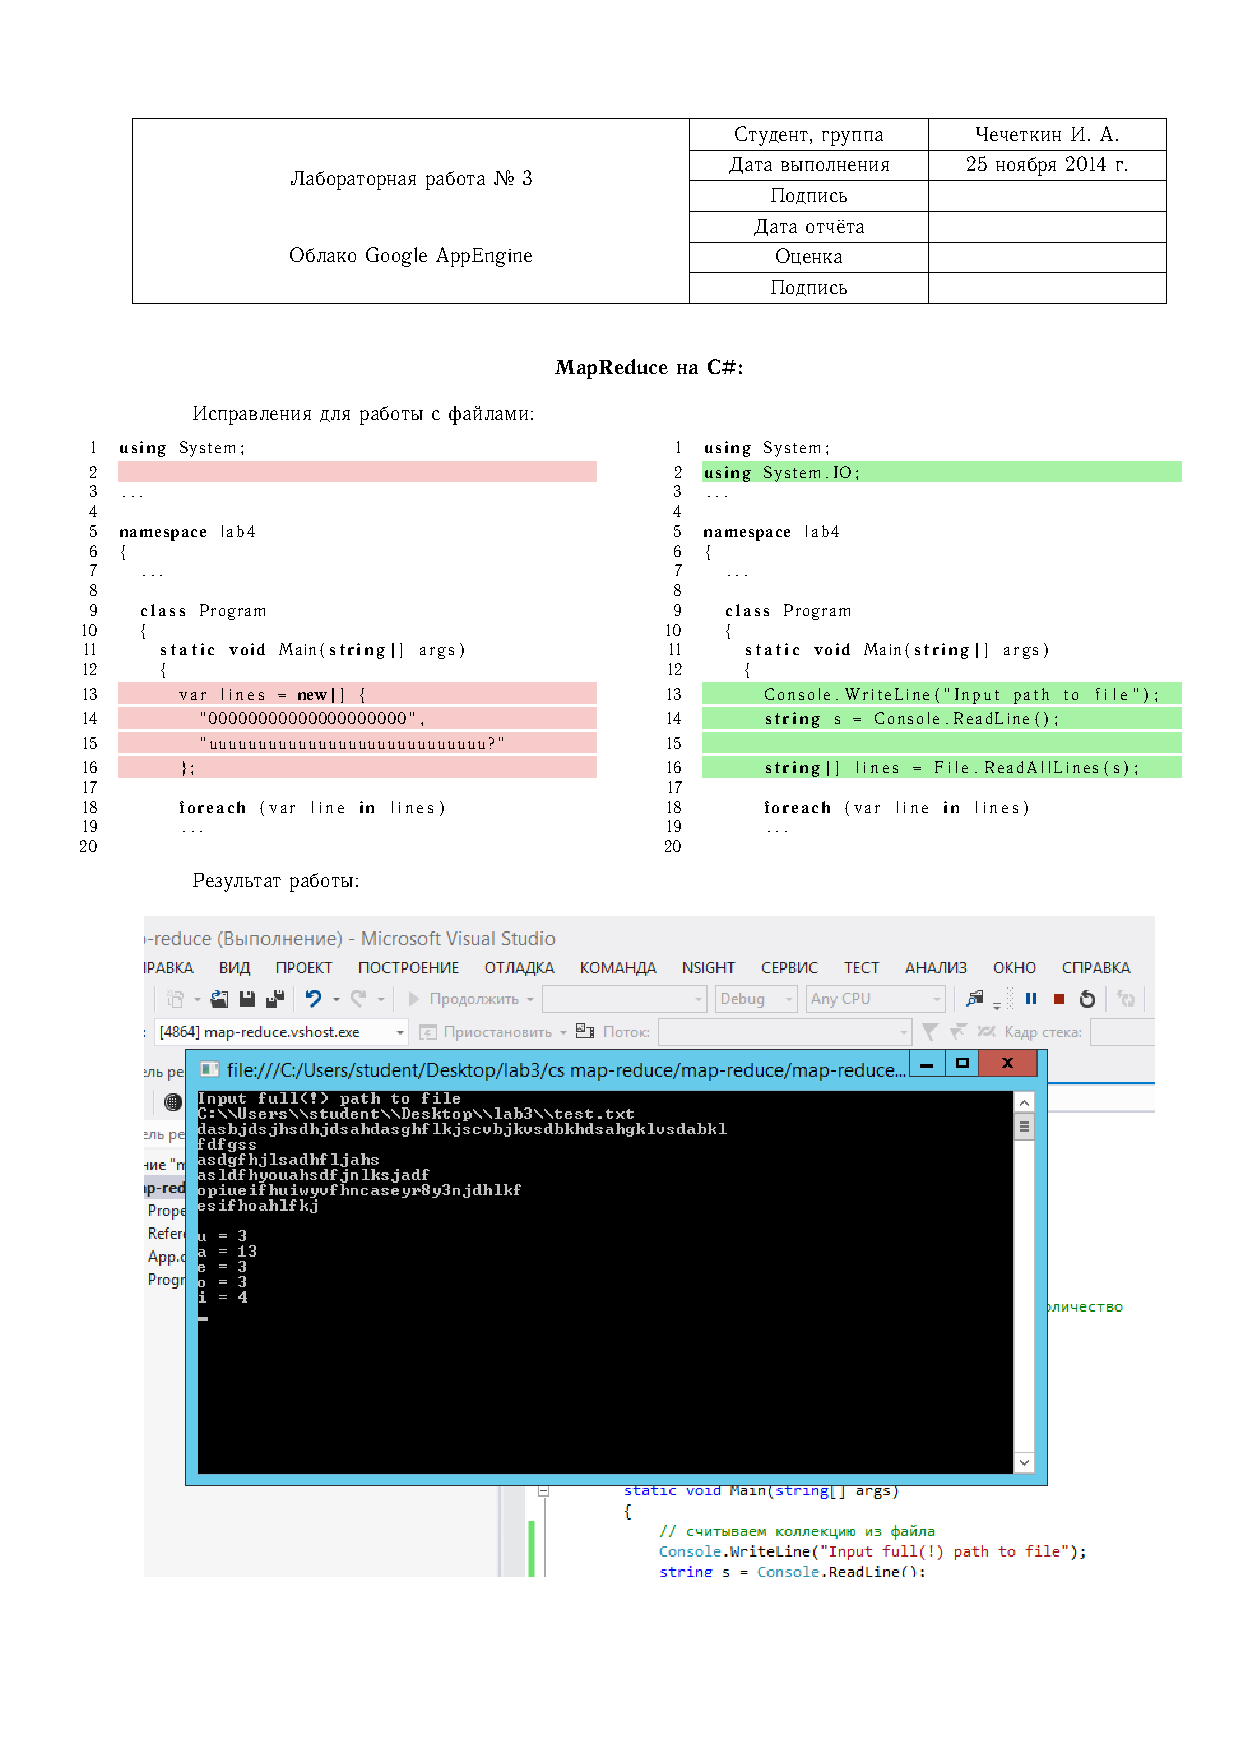
\includegraphics[width=.7\textwidth]{03} \\
    Создание нового приложение в Google App Engine
  \end{figure}
  
  \newpage
  
  \begin{figure}[h!]
    \center
    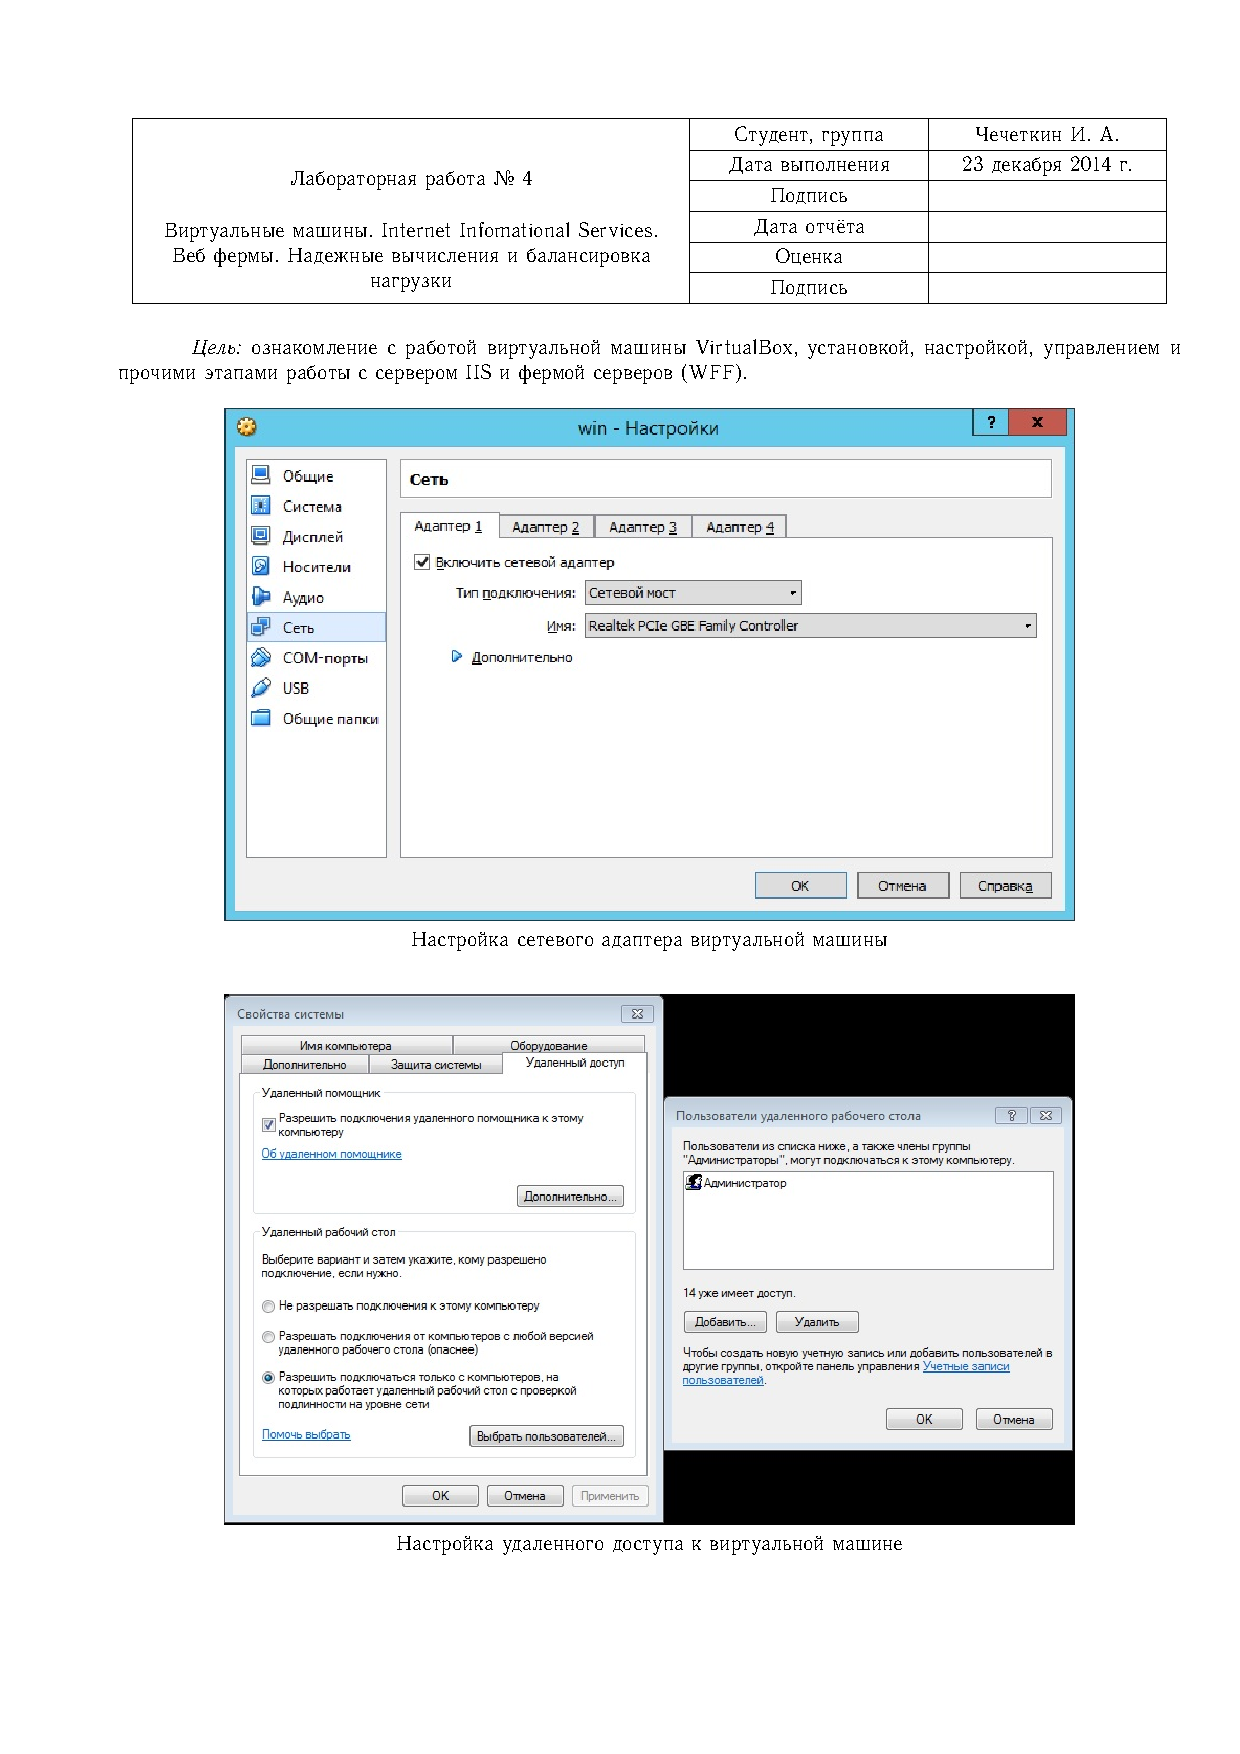
\includegraphics[width=.7\textwidth]{04} \\
    Добавление приложения в Google App Engine
  \end{figure}
  \vspace{-1.5em}
  \begin{figure}[h!]
    \center
    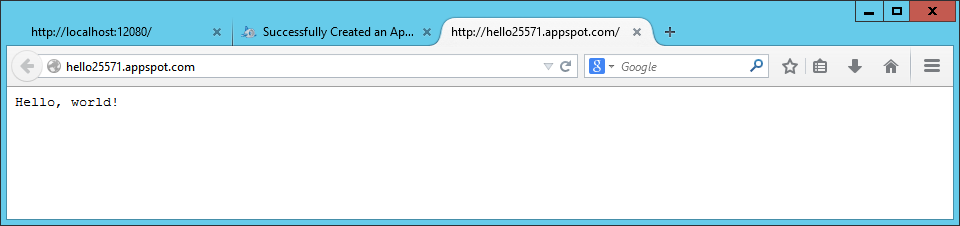
\includegraphics[width=.7\textwidth]{05} \\
    Hello World в облаке Google App Engine
  \end{figure}
  \vspace{-1em}
  
  \begin{center}
    \textbf{MapReduce}
  \end{center}
  \vspace{-1em}
  
  \begin{figure}[h!]
    \center
    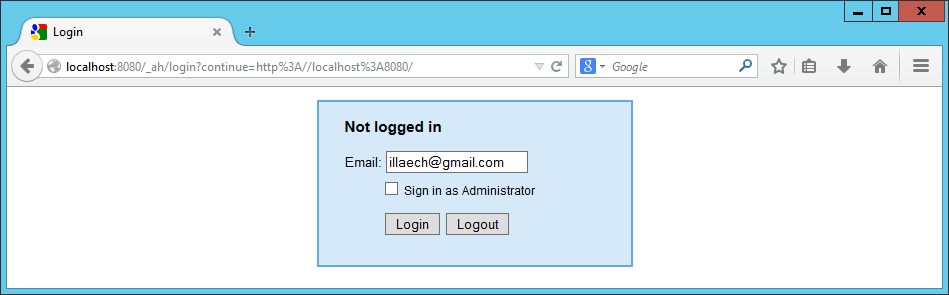
\includegraphics[width=.7\textwidth]{06} \\
    Запрос залогиниться
  \end{figure}
  \vspace{-1.5em}
  \begin{figure}[h!]
    \center
    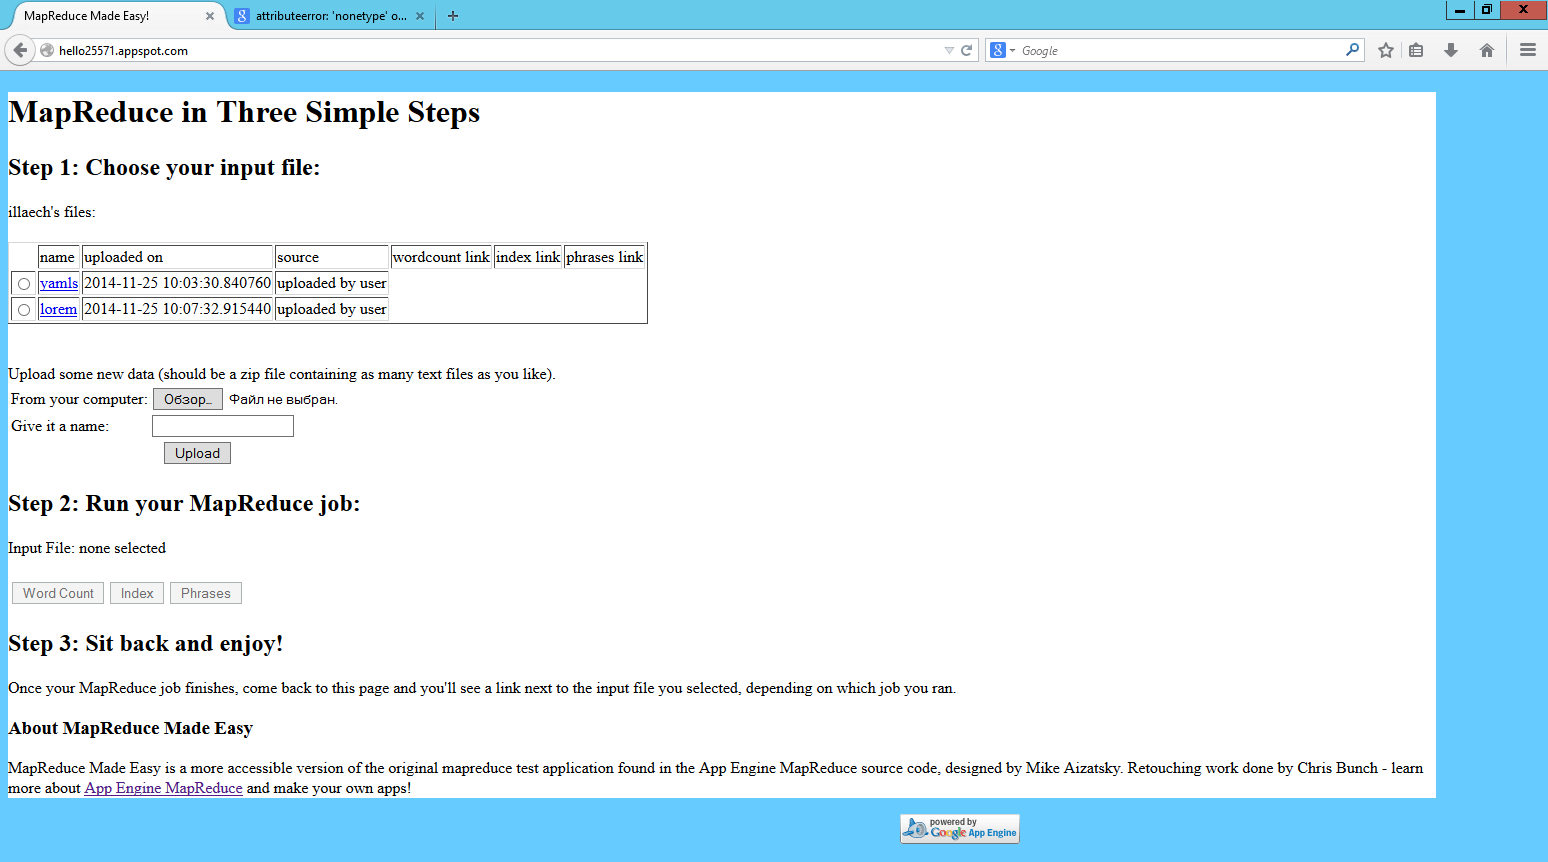
\includegraphics[width=.7\textwidth]{08_0} \\
    Интерфейс
  \end{figure}
  
  \newpage
  
  \begin{figure}[h!]
    \center
    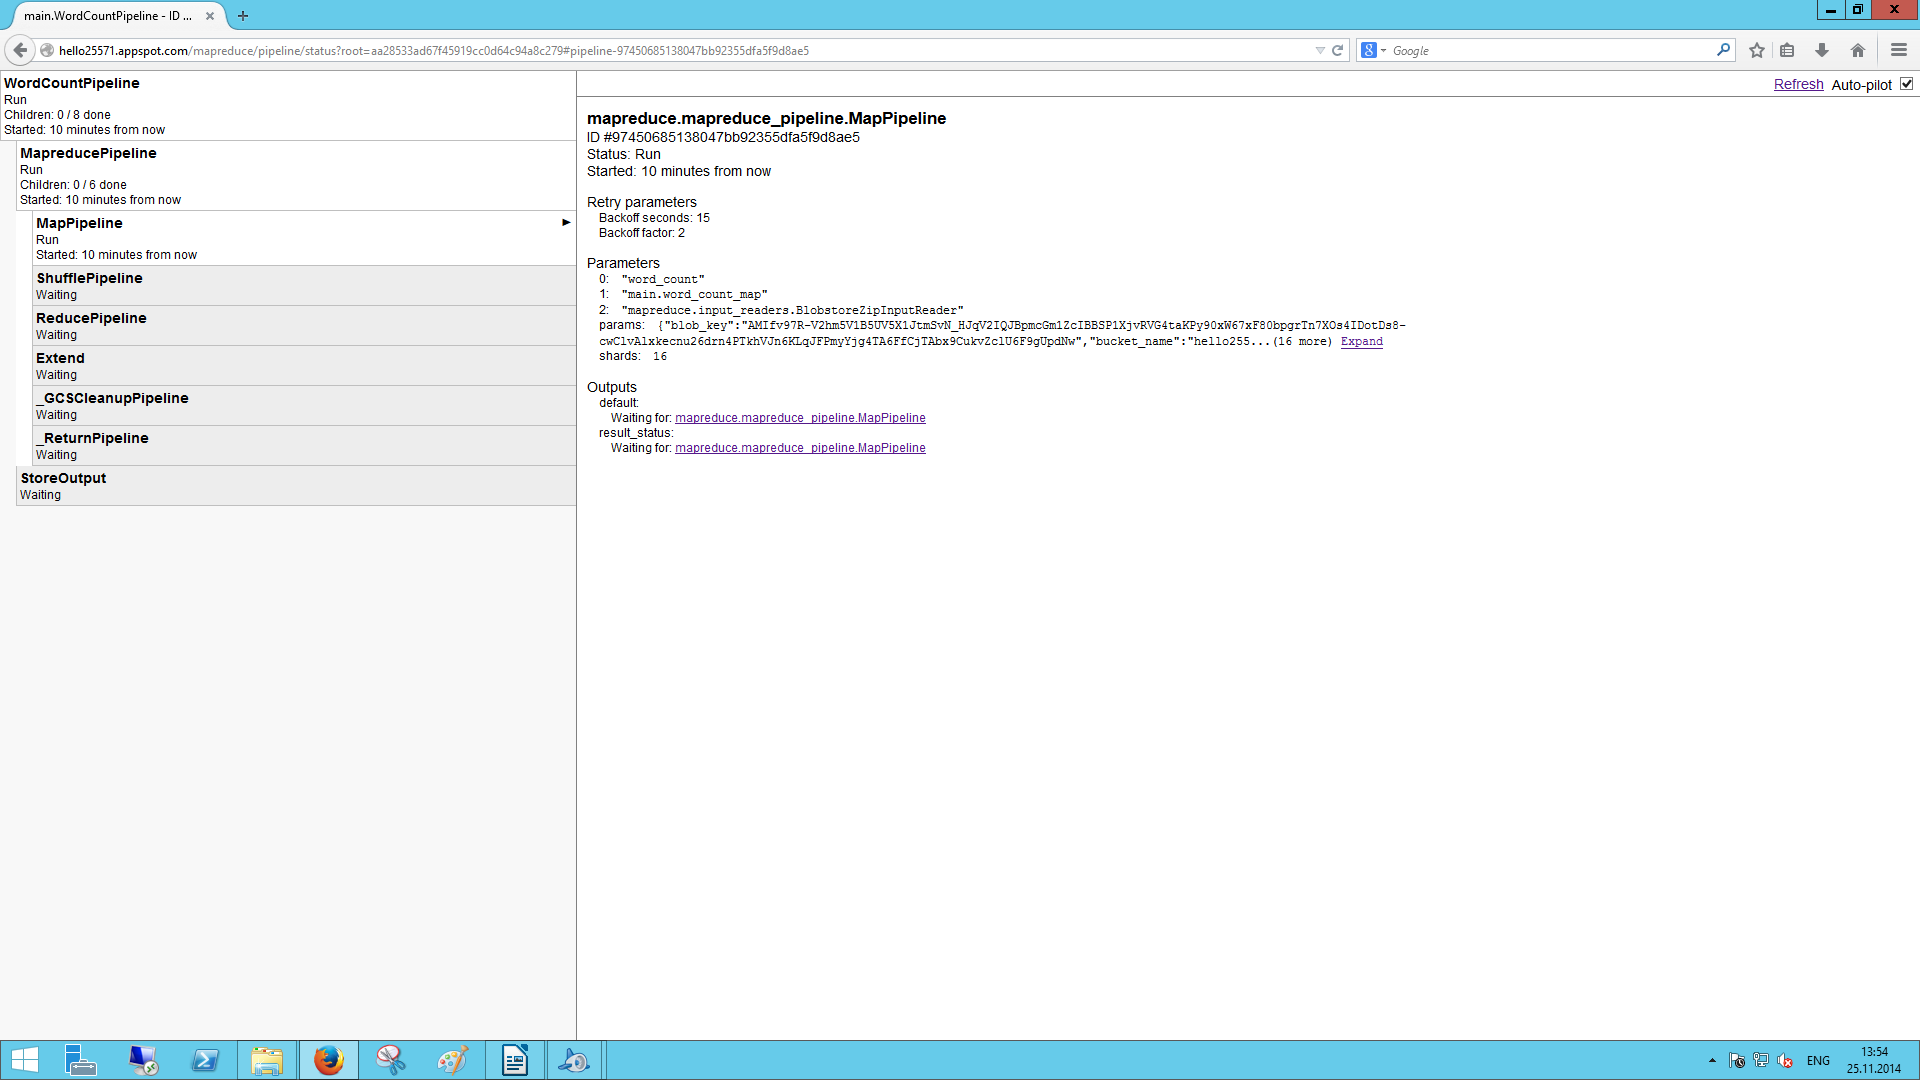
\includegraphics[width=.8\textwidth]{08_1} \\[1ex]
    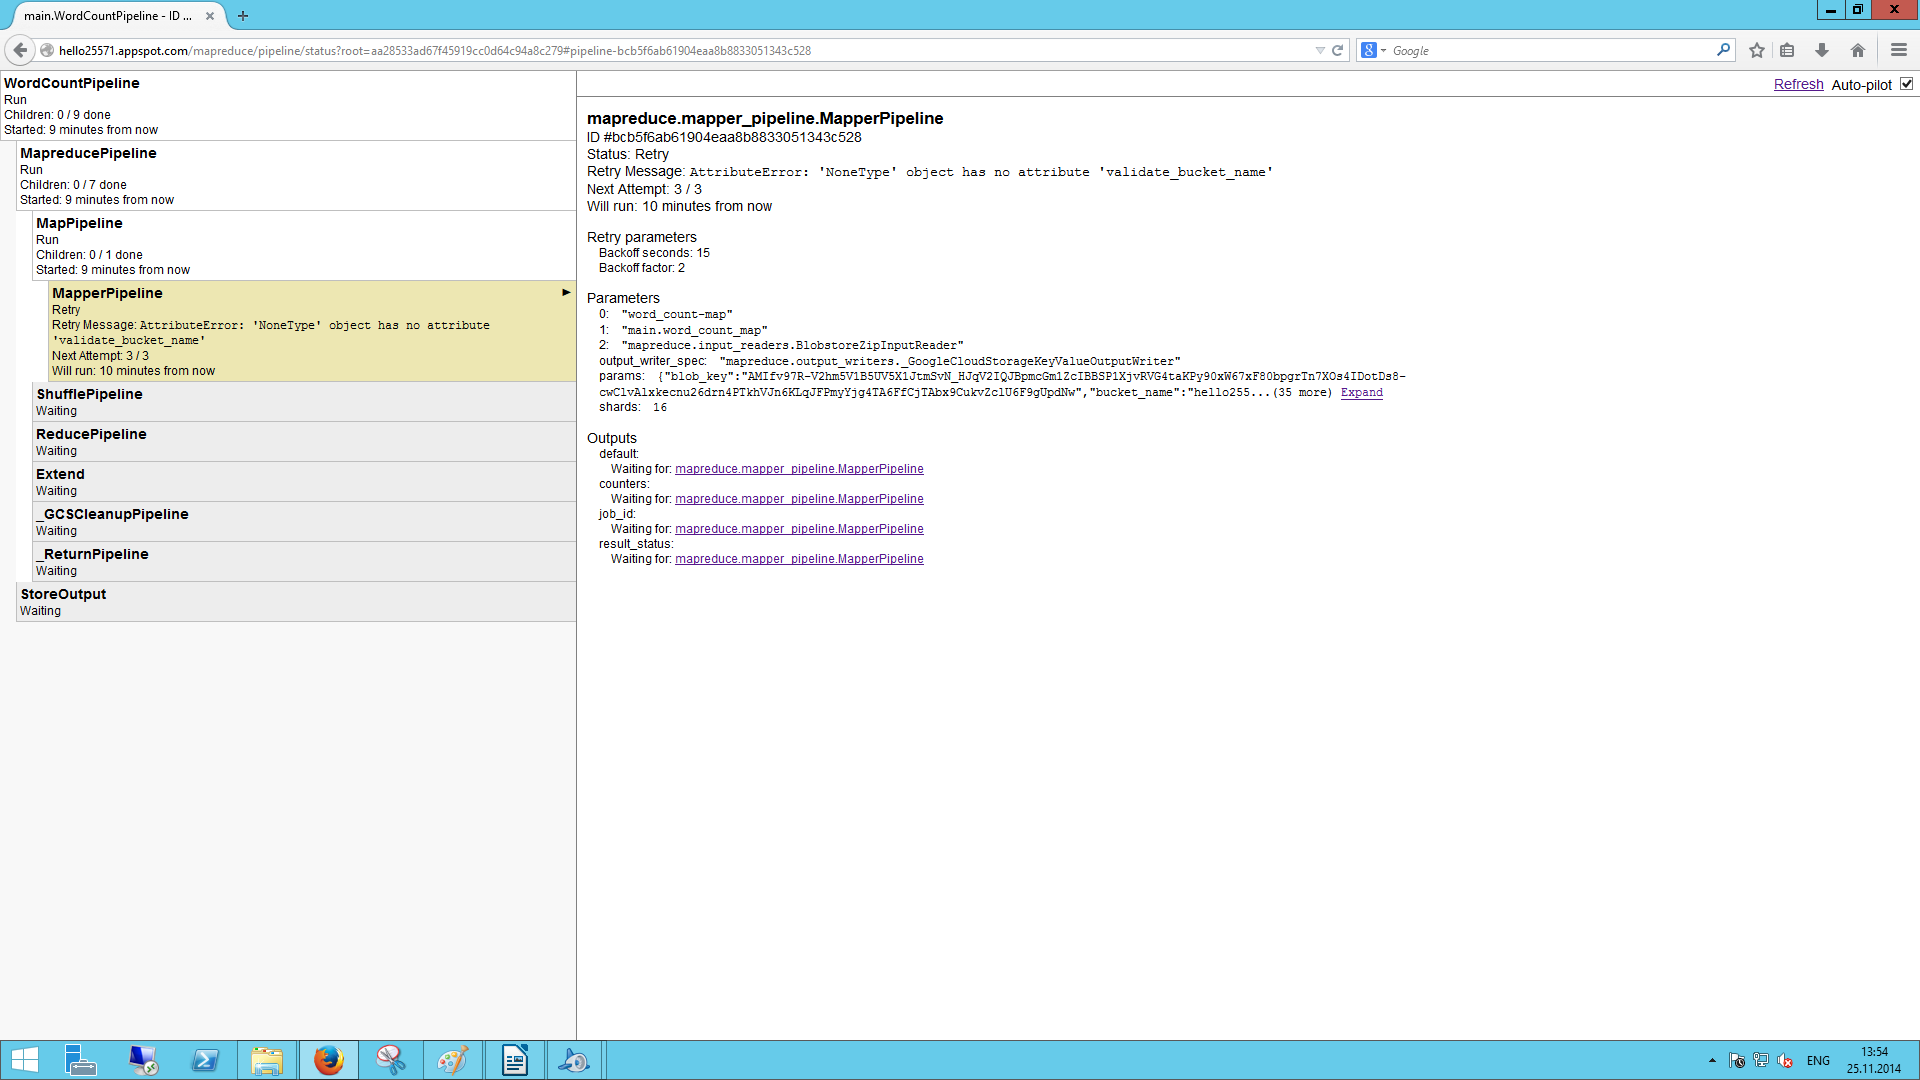
\includegraphics[width=.8\textwidth]{08_2} \\[1ex]
    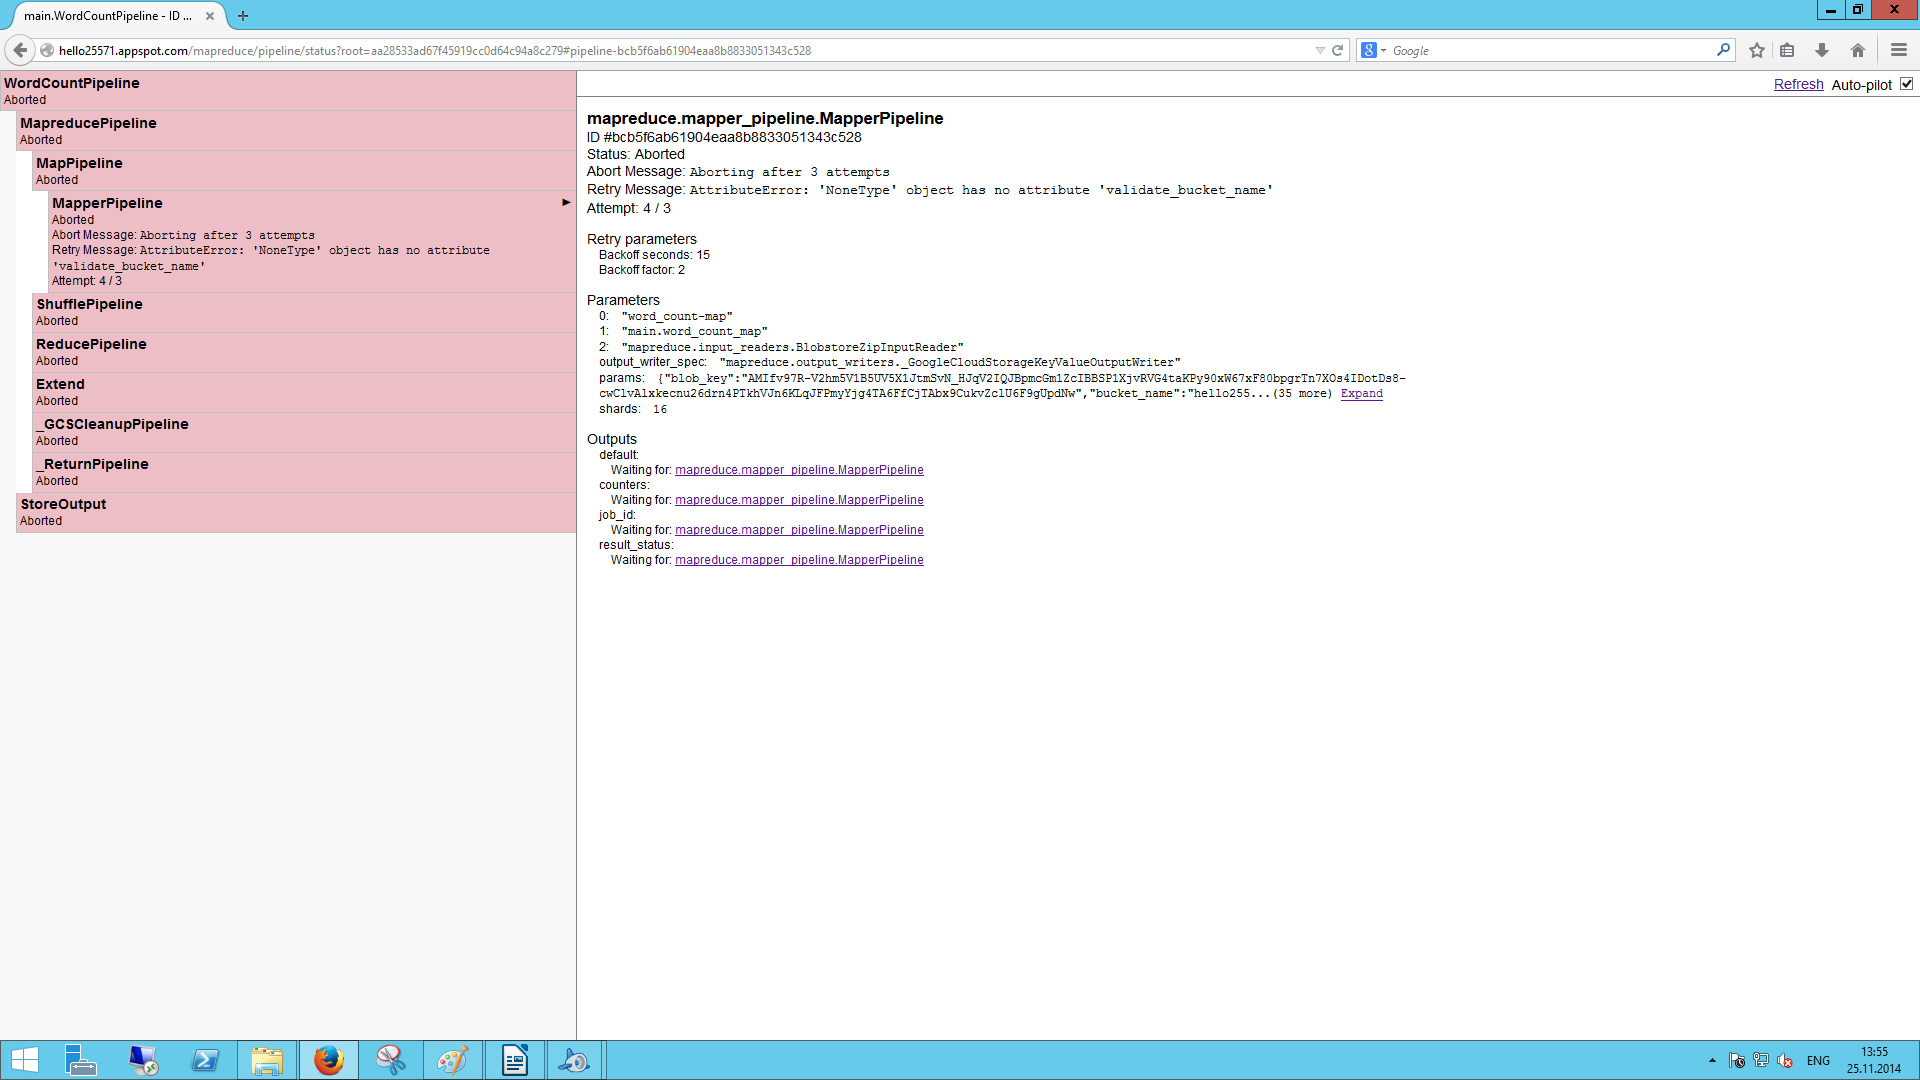
\includegraphics[width=.8\textwidth]{08_3} \\
    Работа алгоритма с ошибкой на выходе
  \end{figure}
  
  
  
\end{document}
